%===============================================================================
% ifacconf.tex 2022-02-11 jpuente  
% 2022-11-11 jpuente change length of abstract
% Template for IFAC meeting papers
% Copyright (c) 2022 International Federation of Automatic Control
%===============================================================================
\documentclass{ifacconf}
\usepackage{graphicx}      % include this line if your document contains 
\usepackage{natbib}        % required for bibliography
\usepackage{amsmath}       % required for align environment
\usepackage{algorithm}
\usepackage{algpseudocode}
\usepackage{tikz}
\usepackage{svg}
%\usepackage{eqnarray}
%\usepackage{tikz}
\usepackage{pgfplots}
%\pgfplotsset{compat=1.18}
\usetikzlibrary{arrows.meta, positioning}
%===============================================================================
\begin{document}
\begin{frontmatter}

\title{Towards Underwater Swarm: A Relative Localization Framework}
% Title, preferably not more than 10 words.

% \thanks[footnoteinfo]{Sponsor and financial support acknowledgment
% goes here. Paper titles should be written in uppercase and lowercase
% letters, not all uppercase.}
\thanks[footnoteinfo]{Corresponding author: Zheng Chen. Associate Professor at Department of Mechanical and Aerospace Engineering, University of Houston, Houston, TX 77004 USA. Email: zchen43@central.uh.edu.}
\author[First]{Muhammad Umar Masood} 
\author[First]{Zheng Chen\thanksref{footnoteinfo}} 
\address[First]{Department of Mechanical and Aerospace Engineering, University of Houston, Houston, TX 77204 USA \\
(emails:mmasood5@cougarnet.uh.edu, zchen43@central.uh.edu)}
\begin{abstract}                % Abstract of 50--100 words
This paper presents a relative localization technique for underwater swarm robotics using received signal strength (RSS) from 433 MHz RF transceivers with directional antennas, fused with inertial measurements from an onboard Inertial Measurement Unit (IMU) via an Extended Kalman Filter (EKF). A leader-follower scenario is simulated in a water tank environment, where the follower fish estimate their position relative to a leader using only RSS and IMU data. The proposed method achieves a reliable estimate of relative distance and orientation, enabling effective formation control. The simulation results demonstrate the feasibility of this approach for distributed underwater swarm coordination.
\end{abstract}
\begin{keyword}
EKF, RSS, IMU, Underwater Swarm, Relative Localization
\end{keyword}
\end{frontmatter}
%===============================================================================
\section{Introduction}
Oceans are the largest ecosystem on the planet, covering more than 70\% of the Earth's surface. Exploration of the resources whether biological, natural, or mineral, in the oceans is still a challenge, due to the harsh underwater environment, high pressure, low visibility, and mainly the lack of reliable communication and localization systems. In the past few decades the researcher focused on developing hardware which can withstand the harsh environment of the oceans \citep{mcleod2012autonomous,Shukla2016}. Communication remains a major challenge where research community has done some considerable growth especially because of the acoustic communication \citep{Su2020,Sun2021}. However, the hardware size of the acoustic communication and sensing is good for large Automated Underwater Vehicles (AUVs) but not for small AUVs or underwater robotic fish.

Reliable localization is a fundamental requirement in a wide range of underwater applications. Techniques such as Simultaneous Localization and Mapping (SLAM), cooperative swarm behaviors, environmental mapping, and multi-agent task distribution all rely on accurate position estimates \citep{Köser2020}. In terrestrial or aerial robotics, these problems are often solved using a combination of GPS, vision-based localization, and robust communication infrastructure. Unfortunately, the underwater environment imposes severe limitations. GPS signals do not penetrate water, optical sensors are limited by turbidity and lighting, and even acoustic methods, though commonly used, are expensive, power-hungry, and often impractical for lightweight or small-scale robotic platforms \citep{Connor2021}.

This challenge is particularly critical in bio-inspired or miniaturized underwater robotic systems, such as robotic fish, which aim to mimic the agility, energy efficiency, and unobtrusiveness of real fish. These platforms, due to size and power constraints, cannot accommodate the bulky and costly navigation systems used by larger autonomous underwater vehicles (AUVs). However, they hold enormous potential for scalable swarm-based applications in constrained or sensitive environments.
To overcome these challenges, a hierarchical system architecture can be envisioned: a large surface or near-surface vessel, such as a remotely operated vehicle (ROV) or a mothership AUV, equipped with high-end localization systems (e.g., GPS, DVL, or acoustic positioning), acts as a reference node or command center. This vessel communicates with a swarm of smaller, low-cost robotic fish that are deployed in the area of interest. These follower robots, while not equipped with precise localization systems, can still navigate and coordinate effectively using lightweight sensors such as radio frequency (RF) transceivers and inertial measurement units (IMU).

Radio frequency has proved to be a workable solution in underwater environment. \cite{Ryecroft2019} implemented 433 MHz communication in raw water. This paper proposes a relative localization technique that fuses Received Signal Strength (RSS) measurements from 433 MHz RF transceivers with inertial data from IMUs using an Extended Kalman Filter (EKF). This fused approach provides each follower robot with an estimate of its relative position and orientation with respect to a reference robot (leader). The leader robot is assumed to have access to global localization (e.g., GPS) and acts as a moving reference for the swarm. The follower robots use the fused relative localization to maintain formation and follow the leader along a desired path.

The proposed technique offers a scalable and low-cost solution to underwater localization, particularly for distributed robotic systems where global positioning is not available. The system is demonstrated in a simulated water tank environment using bio-inspired robotic fish in a leader-follower configuration. Although the focus of this work is on underwater swarm formation, the same methodology is applicable to a wide range of scenarios where a well-localized central agent can guide or coordinate a network of minimally equipped autonomous units.

\section{Localization Estimation}
In this section, two different techniques for relative localization will be discussed, (1) Extended Kalman Filter on IMU data, and (2) Received Signal Strength (RSS) based localization, and then the fusion of both techniques will be discussed. Figure \ref{fig:scheme} shows the black box schematic of the proposed technique. 
\begin{figure}
    \centering
    
\includegraphics[width=1\linewidth]{fig/schematic.png}
    \caption{Schematic of the proposed technique}
    \label{fig:scheme}
\end{figure}
\subsection{Extended Kalman Filter on IMU Data}
The extended Kalman Filter (EKF) is implemented for nonlinear state estimation using acceleration and angular velocity measurements from the IMU, along with optional position updates. The prediction step uses the nonlinear motion model described in Equation~\ref{eq:motionmodel}, and the Jacobian matrix \( F_k \) is computed in each step for linearization. The IMU is attached to the robot in the simulation, which means that its state reflects the true state of the robot. The state of the robot is defined by its position $(x, y)$ and orientation $(\psi)$ in the world frame, as well as its velocities $(u, v, r)$ and their first derivatives in the body frame. The state vector is defined as \( \mathbf{x} = [x, y, \psi, u, v, r, \dot{u}, \dot{v}]^T \), and the measured state is \( \mathbf{z} = [\dot{u}_m, \dot{v}_m, r_m]^T \).
\begin{equation}
    \hat{\mathbf{x}}_{k+1} =
    f(\hat{\mathbf{x}}_k) =
    \begin{bmatrix}
    \hat{x}_k + \hat{u}_k \cos(\hat{\psi}_k) \Delta t - \hat{v}_k \sin(\hat{\psi}_k) \Delta t \\
    \hat{y}_k + \hat{u}_k \sin(\hat{\psi}_k) \Delta t + \hat{v}_k \cos(\hat{\psi}_k) \Delta t \\
    \hat{\psi}_k + \hat{r}_k \Delta t \\
    \hat{u}_k + \hat{\dot{u}}_k \Delta t \\
    \hat{v}_k + \hat{\dot{v}}_k \Delta t \\
    r_{m} \\
    \dot{u}_{m} \\
    \dot{v}_{m}
    \end{bmatrix}
    \label{eq:motionmodel}
\end{equation}
where $\hat{x}_k$, $\hat{y}_k$, $\hat{\psi}_k$, $\hat{u}_k$, $\hat{v}_k$, and $\hat{r}_k$ are the estimated position and orientation of the IMU and $\Delta t$ is the simulation time step.  The noise covariance matrix of the process is defined as:
\begin{equation}
    Q = \mathrm{diag}(Q_{11}, Q_{22}, Q_{33}, Q_{44}, Q_{55}, Q_{66}, Q_{77}, Q_{88})
\end{equation}
where each diagonal entry corresponds to the variance of the respective state variable. The measurement matrix for the IMU is given by:
\begin{equation}
    H_{\text{IMU}} = \begin{bmatrix}
        0 & 0 & 0 & 0 & 0 & 0 & 1 & 0 \\
        0 & 0 & 0 & 0 & 0 & 0 & 0 & 1 \\
        0 & 0 & 0 & 0 & 0 & 1 & 0 & 0
    \end{bmatrix},
\end{equation}
and the corresponding measurement noise covariance is:
\begin{equation}
    R_{\text{IMU}} = \mathrm{diag}(\sigma_{\text{acc}}^2, \sigma_{\text{acc}}^2, \sigma_{\text{gyro}}^2),
\end{equation}
Considering that the accelerometer has symmetric properties in all axes. 

The initial-state covariance matrix is set as:
\begin{equation}
    P = \mathrm{diag}(P_{11}, P_{22}, P_{33}, P_{44}, P_{55}, P_{66}, P_{77}, P_{88})
\end{equation}
The EKF performs two sequential measurement updates: one using IMU data and another using position and heading corrections when available. The general algorithm is shown in Algorithm~\ref{alg:ekf_fused}.
\subsection{Angle of Arrival (AoA) based on Directional Antennas}
Before we can use the relative strength of the signal to estimate the distance from the transmitting leader robotic fish, we need to know the direction from which the transmitted signal is being received. This can be achieved when we have multiple antennas on the receiver (or multiple receivers) and the antennas are directional with some overlap in their beam width. 
\begin{lem}
The angle of arrival (AoA) of the RF signal can be estimated using the RSS data from the multiple antennas on the receiver, provided that the antennas are directional with some overlap in their beam width.
\end{lem}
\begin{lem}
The beam width of half the power of each antenna should be at least $\alpha \geq \frac{360}{N}$, where $N$ is the number of antennas on the receiver.
\end{lem}
The example shown in the work considers four antennas on the receiver, and the half-power beam width of each antenna is $180^{\circ}$. Consider that the receiver position is $(x_r, y_r, z_r)$, and the transmitter position is $(x_t, y_t, z_t)$ and in the planar case $z_r = z_t = 0$, the signal strength in each receiver is indicated by $S_i$ in linear scale, while the antenna $i^{th}$ is directed at an angle $ \theta_i = \psi + \frac{360i}{N}$. $\psi$ is the absolute orientation of the receiver, which would be the same as the orientation of the robot to which the receiver is attached. 
The strength of the signal at each antenna is measured and then sorted in descending order. 
\begin{lem}
Unless the signal is received ideally from $\theta_i$ or $\frac{\theta_i + \theta_{i + 1}}{2}$, no two antennas will have the same signal strength. This being the most general and common case in practice, but in theory there can be some special cases. Considering that the signal is received from an angle $\theta_{rec}$,
\textbf{Case when $\theta_{rec} = \theta_i$}: The signal strength of the first antenna in the sorted list will be the highest, and the signal strength of the second and third will be the same ($S{i + 1} = S_{i - 1}$).
\textbf{Case when $\theta_{rec} = \frac{\theta_i + \theta_{i + 1}}{2}$}: The signal strength of the first antenna and the second antenna in the sorted list will be the highest, and the other will be lower.
\end{lem}
\textbf{Note:} As the simulation is realistic and white noise is added to the signal strength, the signal strength of the antennas will not be exactly the same and the described algorithm will always work. It is still a good idea to implement a check to see if their is any division by zero in the algorithm because of the two cases described above. 
Let us take the first two antennas in the sorted list, the highest valued as reference $S_{ref}$ and the adjacent one $S_{adj}$. For $S_{ref} = S_{i}$, the adjacent antenna will be $S_{i + 1}$ or $S_{i - 1}$. The subscripts $ref$ and $adj$ can be used as value numbers that show the actual antenna index.
\textbf{Example:} The signal is received from $120^{\circ}$, the sorted list will be $S_1 > S_2 > S_0 > S_4$, which means $ref = 1$ and $adj = 2$. 
The relative angle of arrival can be calculated as follows:
\begin{equation}
    \theta_{rel} = -\frac{1}{2} (90 + \frac{\alpha^2}{90} \frac{(S_{ratio})_{dB}}{12}),
    \label{eq:rel}
\end{equation}
where $S_{ratio} = 10 \log_{10}(\frac{S_{adj}}{S_{ref}})$, and $\alpha$ is the half-power beam-width of the antenna. The relative angle of arrival is the angle between the direction of the receiver $ref$ and the direction of the transmitter. The angle of arrival (AoA) would be
\begin{equation}
    \theta_{AoA} = \theta_{ref} + \theta_{rel}(ref - adj).
    \label{eq:aoa}
\end{equation}
In the final equation above, $ref - adj$ tells whether the adjacent antenna is the right neighbor or the left neighbor of the reference antenna.  
\subsection{RSS based Localization}
Once the angle of arrival (AoA) is calculated, the distance between the transmitter and the receiver can be estimated using the RSS value on any of the receiving antennas. For example, taking the first antenna in the sorted list, the distance between the transmitter and the receiver can be estimated as follows:
\begin{equation}
    d_{rss} = \left\|(\frac{(P_t)_{dB} + (G(\theta_{rel}))_{dB}-(S_{ref})_{dB}}{0.0173 \sqrt{f_{rf} \times \sigma}})\right\|,
\end{equation}
Both the distance and angle are estimated, so the relative location of the transmitter can be estimated as follows:
\begin{equation}
    x_{tx} = x_r + d_{rss} \cos(\theta_{AoA}),
    y_{tx} = y_r + d_{rss} \sin(\theta_{AoA}).
\end{equation}

\subsection{Fusion of IMU and RSS based Localization}
The extended Kalman Filter (EKF) is used to fuse measurements from both the IMU and the RSS-based localization system to estimate the robot's full state, including position and orientation. Sensor fusion is performed through two sequential update steps within a single EKF framework. The first update incorporates raw IMU data, such as linear accelerations and yaw rates, using the measurement matrix \( H_{\text{IMU}} \) and the associated noise covariance \( R_{\text{IMU}} \). The second update refines the state estimate using position and heading information obtained from RSS-based localization, through a separate measurement model defined by \( H_{\text{pos}} \) and a corresponding confidence matrix \( R_{\text{pos}} \).

Unlike \( R_{\text{IMU}} \), which reflects direct sensor noise, \( R_{\text{pos}} \) captures the uncertainty in the position estimate inferred from the RSS signals. These updates are applied sequentially, as described in Algorithm~\ref{alg:ekf_fused}, ensuring a consistent and flexible fusion of heterogeneous data sources within the EKF pipeline.
    \begin{algorithm}
    \caption{Extended Kalman Filter with IMU and Position Correction}
    \label{alg:ekf_fused}
    \begin{algorithmic}[1]
        \State Initialize $\hat{\mathbf{x}}, P, Q, R_{\text{IMU}}, R_{\text{pos}}$
        \While{simulation is running}
            \State \textbf{Prediction Step:}
            \State \hspace{1em} Compute $\hat{\mathbf{x}}_{k+1} = f(\hat{\mathbf{x}}_k)$
            \State \hspace{1em} Compute $F_k = \frac{\partial f}{\partial \mathbf{x}} \big|_{\hat{\mathbf{x}}_k}$
            \State \hspace{1em} Update $P \gets F_k P F_k^\top + Q$

            \State \textbf{IMU Measurement Update (if available):}
            \State \hspace{1em} Measure $\mathbf{z}_{IMU}$
            \State \hspace{1em} Compute $y_{\text{IMU}} = \mathbf{z}_{\text{IMU}} - H_{\text{IMU}} \hat{\mathbf{x}}$
            \State \hspace{1em} Compute $K = P H_{\text{IMU}}^\top (H_{\text{IMU}} P H_{\text{IMU}}^\top + R_{\text{IMU}})^{-1}$
            \State \hspace{1em} Update $\hat{\mathbf{x}} \gets \hat{\mathbf{x}} + K y_{\text{IMU}}$
            \State \hspace{1em} Update $P \gets (I - K H_{\text{IMU}}) P$
            \State \hspace{1em} (Optional) Store $\hat{\mathbf{x}}_{IMU} \gets \hat{\mathbf{x}}$
            

            \State \textbf{RSS Position Update:}
            \State \hspace{1em} Compute $y_{\text{pos}} = \mathbf{z}_{\text{pos}} - H_{\text{pos}} \hat{\mathbf{x}}$
            \State \hspace{1em} Compute $K = P H_{\text{pos}}^\top (H_{\text{pos}} P H_{\text{pos}}^\top + R_{\text{pos}})^{-1}$
            \State \hspace{1em} Update $\hat{\mathbf{x}} \gets \hat{\mathbf{x}} + K y_{\text{pos}}$
            \State \hspace{1em} Update $P \gets (I - K H_{\text{pos}}) P$
        \EndWhile
    \end{algorithmic}
\end{algorithm}
\section{Simulation Environment}
The simulation environment, created using the VPython library, consists of a water tank with a leader robot, a follower robot, and a pipeline at the bottom of the tank. Both robots are bioinspired robotic fish that have the dynamic model described in one of the previous works by the authors in \cite{Masood2025}. A complete non-linear dynamic model of the robotic fish is numerically solved in the simulation. An inertial measurement unit (IMU) and radio frequency transmitter and receivers are also modeled with specified parameters to realistically simulate the system to test the estimation algorithm. 

\subsection{Leader Robot}
The leader robot is equipped with a radio frequency transmitter and receiver, an IMU, a GPS, and a camera. The leader robot is programmed to track the pipeline in the bottom of the tank. The leader robot is considered to have higher capability in terms of sensors and processing power, compared to the follower robot(s). The leader robotic fish is capable of autonomously tracking the pipeline, which is shown in detail in \cite{Masood2025}. 
\subsection{Follower Robot}
The follower robot is equipped with a radio frequency transmitter and receiver and an IMU. The follower robot is programmed to follow the leader robot maintaining a constant distance. 
\subsection{Pipeline}
The pipeline is a straight line on the bottom of the tank. The pipeline is used as a reference for the leader robot to follow. The pipeline is considered to be a straight line, but it can be modeled as a curve or a complex shape for more realistic simulation.

\subsection{Environment}
An simulated environment class is also designed, which keeps the testing water pool, pipeline, robots, and virtually, the RF signal strength in 3D space based on the attenuation of RF signal in the environment.

\subsection{RSS Unit}
The RSS unit is the name given to the sensor node presented, which contains an RF transmitter and receiver with four antennas. The RSS unit is mounted on the leader and follower robots. The RSS unit is used to measure the RSS of the RF signals between the leader and follower robots. The RSS data are used to estimate the distance between the leader and follower robots. The RSS data are fused with the IMU data with estimation through the extended Kalman filter (EKF).

\subsubsection{Transmitter}
The transmitter in each RSS unit transmits the RF signal of defined frequency and power. The transmitter updates the signal strength of the specific frequency band in the environment class. The signal strength (in $dB$) at any point in the environment $(x_e, y_e, z_e)$ is calculated as follows:
\begin{equation}
    S_e = P_t + G_t - P_{loss},
\end{equation}
where $S_e$ is the signal strength at the point $(x_e, y_e, z_e)$, $P_t$ is the transmitted power, and $P_loss$ is the path loss of the RF signal. The path loss of the RF signal is calculated as follows:
\begin{equation}
    P_{loss} = \alpha_w \times d,
\end{equation}
where $\alpha_w$ is the water attenuation coefficient in $dB/m$, and $d$ is the distance between the transmitter and the receiver, defined as
\begin{equation}
    d = \sqrt{(x_t - x_e)^2 + (y_t - y_e)^2 + (z_t - z_e)^2},
\end{equation}
and $(x_e, y_e, z_e)$ are the coordinates of the transmitter and any point in the environment, respectively. The water attenuation coefficient is a function of the frequency of the RF signal, the salinity of the water, and the temperature of the water. The water attenuation coefficient is calculated as described in \cite{vk5br1987}:
\begin{equation}
    \alpha_w = 0.0173 \sqrt{f_{rf} \times \sigma},
\end{equation}
where $f_{rf}$ is the frequency of the RF signal in $Hz$, and $\sigma$ is the conductivity of water in siemens per meter $S/m$. 

\subsubsection{Receiver}
The receiver in each RSS unit receives the RF signal from multiple directions. For the purpose of this study, we have considered four antennas on each RSS unit. For $N$ antennas, the angular separation between the antennas is $ \theta_i - \theta_{i-1} = 360/N$, when $i = 1, 2, 3, ..., N$ and $\theta_i$ is the direction of the $i^{th}$ antenna. 
Each antenna is a directional antenna with a gain of $G_r(\theta)$ which is defined in \cite{Stutzman1998, stutzman2012antenna} as follows:
\begin{equation}
    G_r(\theta) = G_{max} - 12 \times \frac{\theta}{\alpha}^2,
\end{equation}
where $G_{max}$ is the maximum gain of the antenna, $\theta$ is the angle of the antenna with respect to the direction of the RF signal, and $\alpha$ is the beam width of the antenna which is defined as the angle at which the antenna gain is reduced by half, that is, $G_r(\alpha) = G_{max}/2$ and $\alpha = 2 \time \theta_{3dB}$. $\theta_{3dB}$ is the half power beam-width of the antenna. The received signal strength at the receiver is calculated as follows:
\begin{equation}
    S_r = S_e + G_r(\theta).
\end{equation}
Note that the received signal strength is calculated for each antenna separately and the units are in $dB$. Figure \ref{fig:RSS} shows the RSS unit with a receiver with one antenna and an omnidirectional transmitter in the testing water tank environment, and their respective notations for angles, distances and signal strength.
\begin{figure}
    \centering
    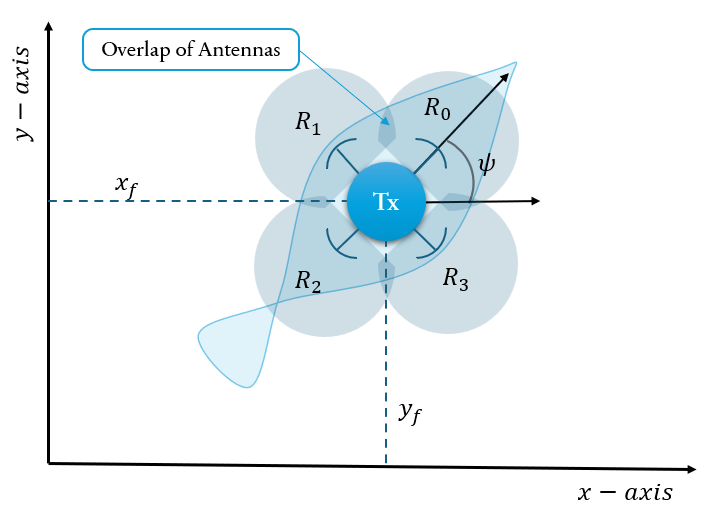
\includegraphics[width=0.5\textwidth]{fig/RSS.png}
    \caption{RSS unit mounted on a robotic fish with an omnidirectional transmitter and four directional antennas, and their respective notations for angles, distances and signal strength.}
    \label{fig:RSS}
\end{figure}

\subsection{IMU Sensor}
Each IMU sensor contains a three-axis accelerometer and a three-axis gyroscope, which are used to measure the linear acceleration and angular velocity of the robots. The IMU data are used to estimate the position and orientation of the robots. The IMU data are fused with the RSS data with estimation through the extended Kalman filter (EKF). Following most of the commercially available IMUs, the IMU sensor is modeled to have white noise and drift in the measurements. The IMU is attached to the robot, hence the actual position of the IMU is always the actual position of the robot. The measured acceleration and angular velocity will be as follows:
\begin{equation}
    \begin{aligned}
    \ddot{x}_m &= \ddot{x} + \eta_{acc} + \nu_{acc}, \\
    \ddot{y}_m &= \ddot{y} + \eta_{acc} + \nu_{acc}, \\
    \dot{\psi}_m &= \dot{\theta} + \eta_{gyro} + \nu_{gyro}.
    \end{aligned}
\end{equation}
where $\ddot{x}_m$, $\ddot{y}_m$, and $\dot{\psi}_m$ are the acceleration measured in the x and y directions and the angular velocity, respectively. $\ddot{x}$, $\ddot{y}$, and $\dot{\psi}$ are the actual acceleration in the x and y directions, and the angular velocity, respectively. $\eta_{acc}$ and $\eta_{gyro}$ are the white noise in the acceleration and angular velocity measurements, respectively. $\nu_{acc}$ and $\nu_{gyro}$ are the drifts in the acceleration and angular velocity measurements, respectively. Figure \ref{fig:IMU} shows the values of the IMU sensor, when it is in rest position in the presence of gravity.
\begin{figure}
    \centering
    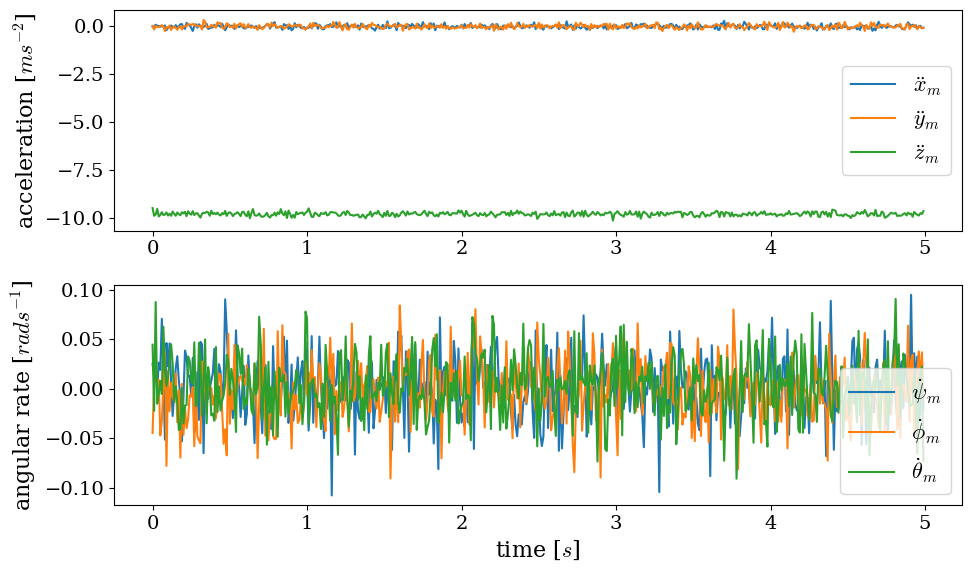
\includegraphics[width=0.45\textwidth]{fig/IMU.png}
    \caption{IMU sensor values, when it is in rest position in the presence of gravity.}
    \label{fig:IMU}
\end{figure}

\section{Formation Control and Results}
\subsection{Localization Performance}
Before demonstrating formation control, we evaluated the performance of individual localization components that contribute to the relative positioning of the fused. Figure~\ref{fig:IMU_localization} illustrates a comparison between the estimated positions using the IMU-only, RSS-only, and the proposed fused EKF approach against the actual ground truth position of the follower robotic fish. 

The top subplot shows the 2D position trajectories, while the bottom subplot presents the corresponding estimation errors over time. The IMU-only estimate (green) exhibits cumulative drift over time due to the integration of noisy accelerations. The RSS-based estimate (orange) is more stable but exhibits higher frequency fluctuations due to the uncertainty of directional estimation. In contrast, the fused EKF estimate (blue) maintains accuracy by combining the short-term precision of the IMU with the long-term stability of RSS measurements. The error plot clearly demonstrates that the fused estimate consistently outperforms both individual methods in terms of accuracy and robustness.
\begin{figure}
    \centering
    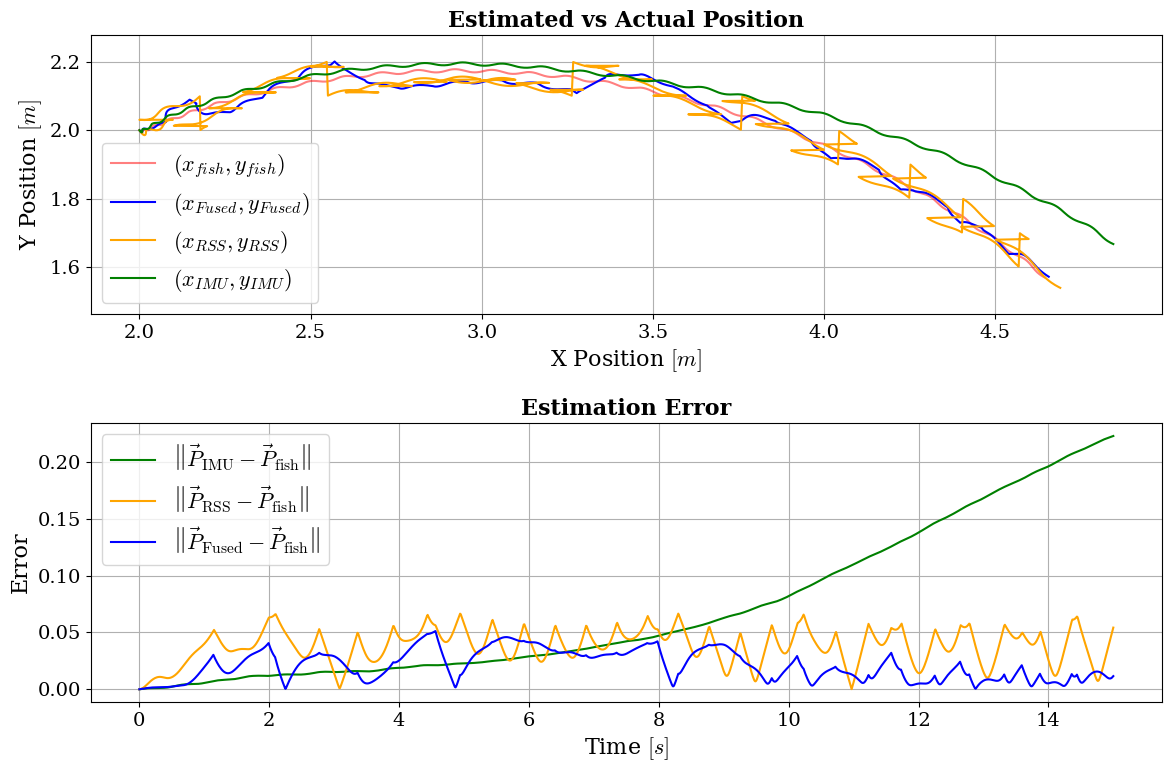
\includegraphics[width=0.45\textwidth]{fig/IMU_localization.png}
    \caption{Comparison of estimated and actual position using IMU-only, RSS-only, and fused EKF-based localization. The bottom subplot shows the corresponding estimation error over time.}
    \label{fig:IMU_localization}
\end{figure}

\subsection{Leader-Follower Formation Control}
To validate the practical utility of the proposed localization method, we simulate a leader-follower formation control scenario relevant to underwater pipeline inspection. In this setup, a leader robotic fish - equipped with GPS, a camera, and inertial sensors - follows a predefined path along the tank floor. The follower robotic fish, equipped only with an IMU and an RSS-based localization unit, estimates its relative position and orientation with respect to the leader and maintains formation accordingly. For this experiment $d_{ref}$ is set to 1 m. 

Each follower fish is controlled via two actuation signals: the tail beat frequency, which regulates forward propulsion, and the tail angle, which controls steering. A proportional controller is implemented to regulate both distance and alignment. Due to the nonlinear dynamics and oscillatory behavior of the fish, we adopt a simplified control strategy to focus on evaluating the effectiveness of relative localization.
The control laws are defined as follows:
\begin{equation}
u_{\text{tail}} = 
\begin{cases}
k_p (d_{\text{Fused}} - d_{\text{ref}}), & \text{if } d_{\text{Fused}} > d_{\text{ref}} \\
0, & \text{otherwise}
\end{cases},
\end{equation}
\begin{equation}
\delta_{\text{tail}} = k_\delta \cdot \theta_{\text{AoA}},
\end{equation}
where $d_{\text{Fused}}$ is the estimated distance between the leader and the follower, $d_{\text{ref}}$ is the desired inter-agent distance, $\theta_{\text{AoA}}$ is the angle of approach between the follower and the leader, and $k_p$, $k_\delta$ are proportional control gains. The controller ensures basic formation-keeping behavior by adjusting forward propulsion and turning.

This setup, implemented in a simulation environment, demonstrates that even with a minimal control strategy, the swarm is capable of maintaining formation and tracking the pipeline. This validates the usefulness of the relative localization technique for distributed coordination in underwater robotic swarms. Figure \ref{fig:formation_control} shows the formation control of the robotic fish swarm using the proposed relative localization technique. A complete simulation framework is implemented with a testing water tank, a pipeline in the bottom, and the robotic leader fish tracking the pipeline while the robotic follower fish maintaining a constant distance from the leader. The water tank is shown in light blue.
\begin{figure}
    \centering
    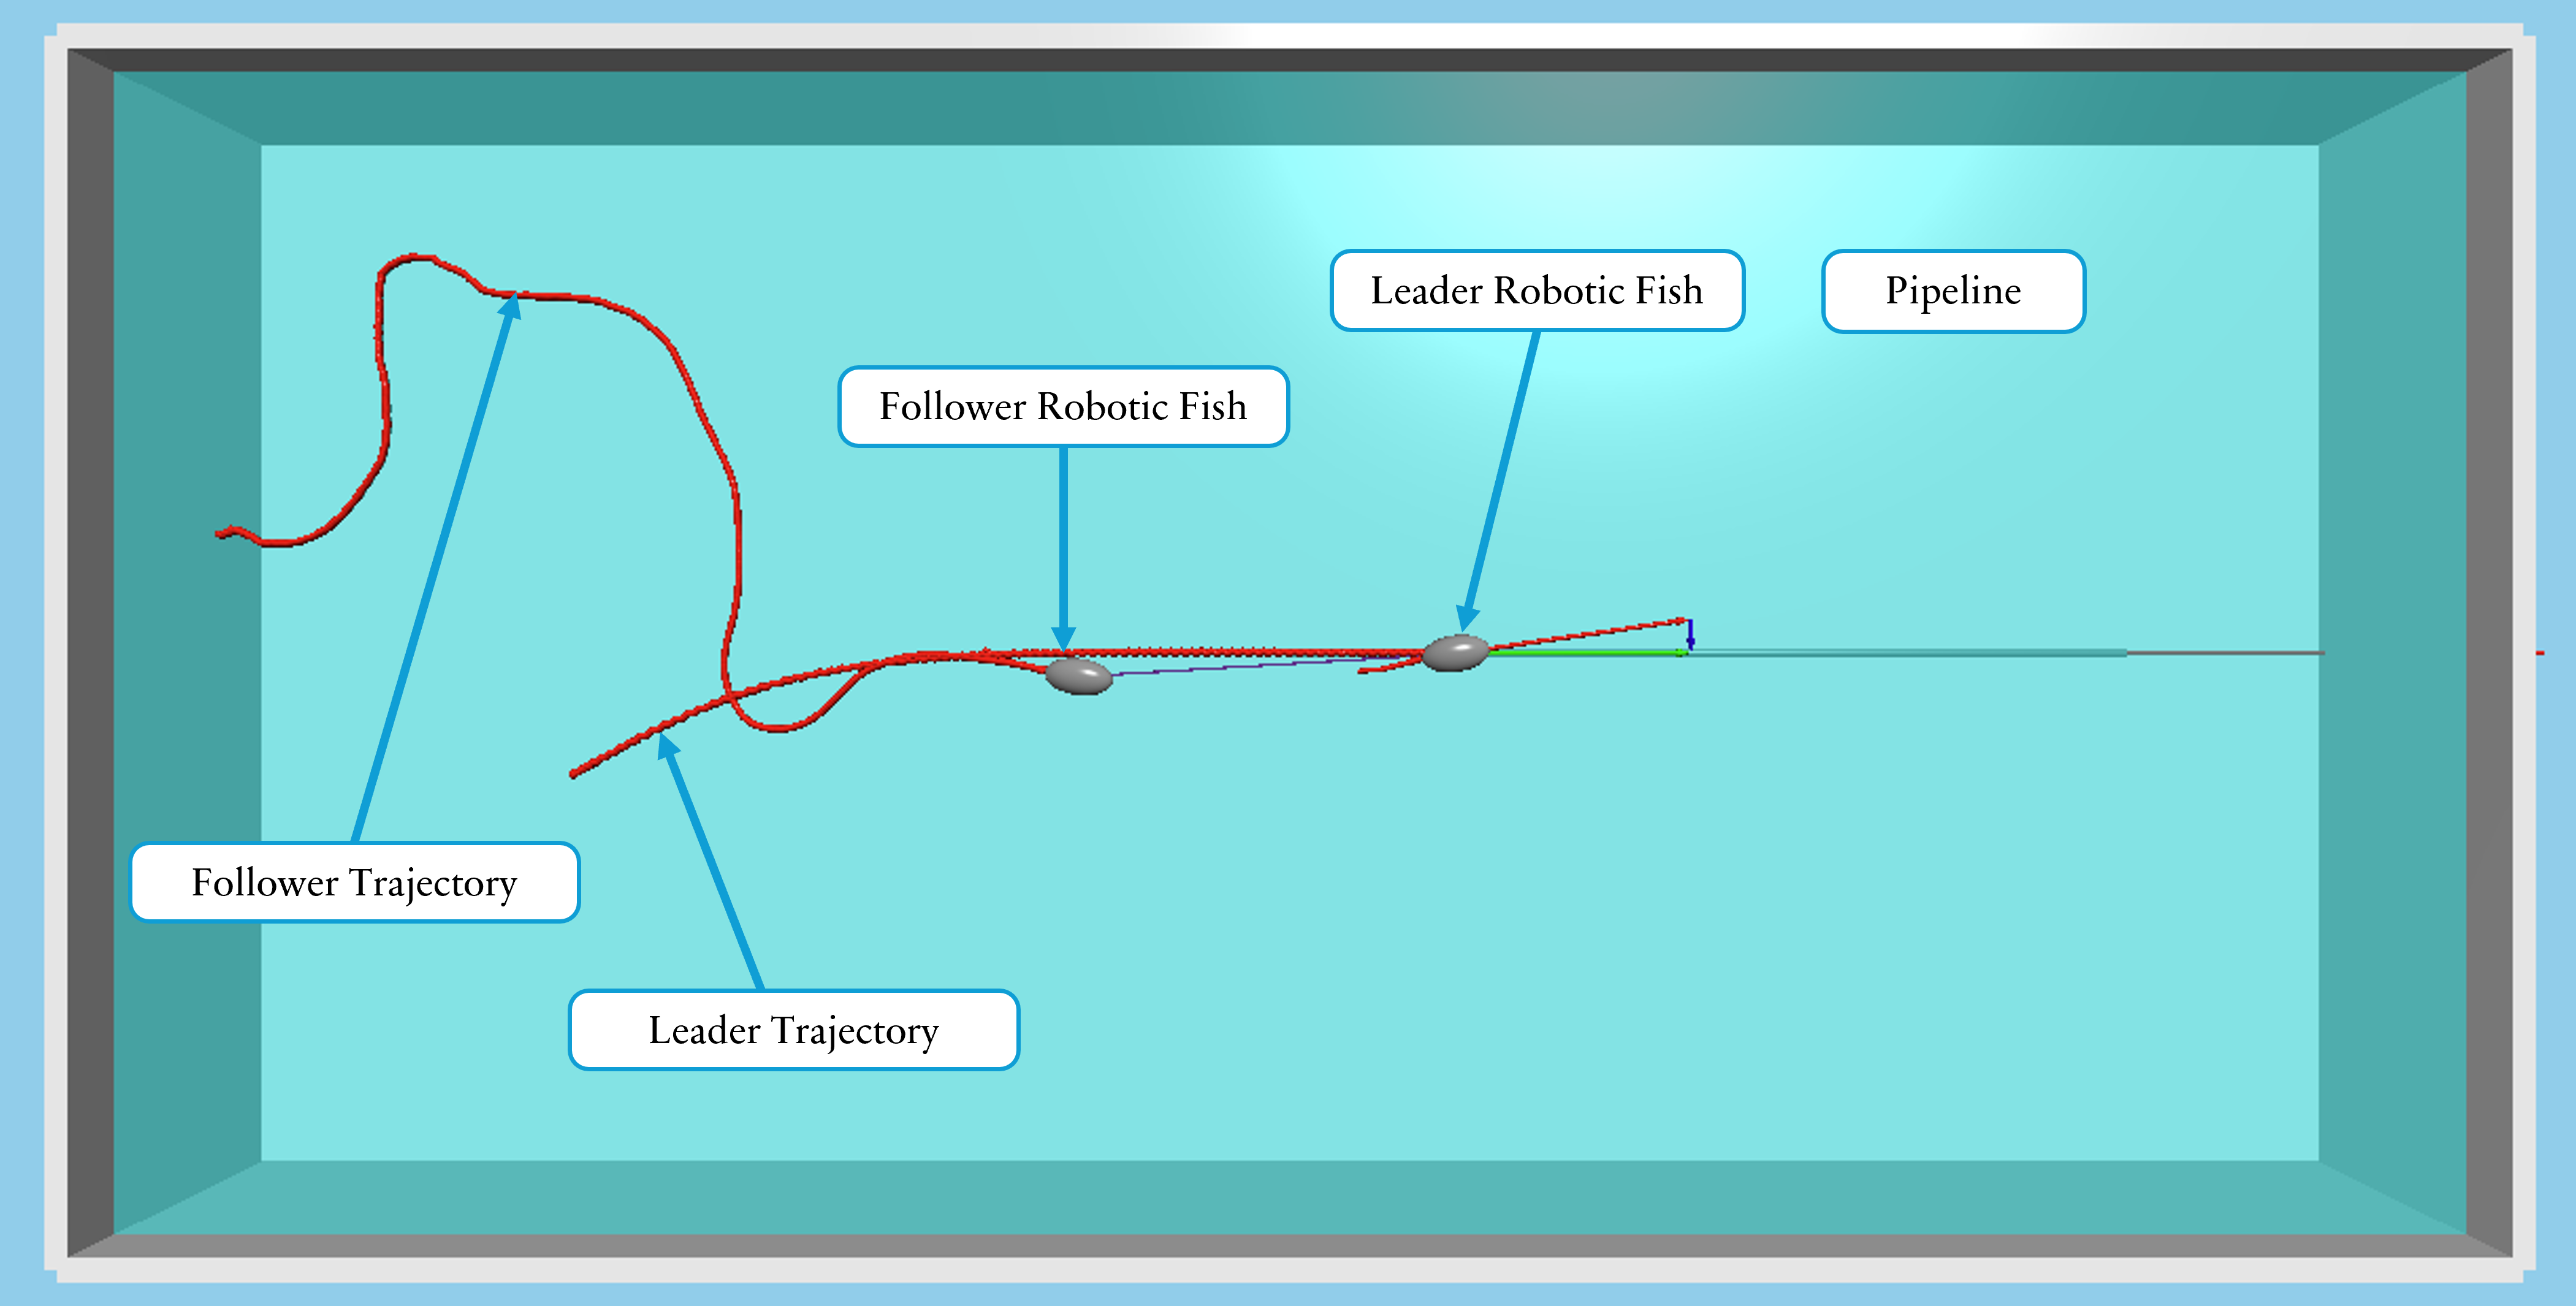
\includegraphics[width=0.45\textwidth]{fig/Formation_pool_annotated.png}
    \caption{Formation control of the robotic fish swarm using the proposed relative localization technique.}
    \label{fig:formation_control}
\end{figure}

Due to inherent noise in the measurements of the RSS and IMU sensors, the follower fish may not always maintain a constant inter-agent distance from the leader, but a detailed analysis shows that the distance and the relative angle converge to the desired values. 
Figure~\ref{fig:formation_errors} illustrates the performance of the relative localization system by comparing the estimated and ground-truth values for the distance and angle between the robotic fish follower and the leader. 
\begin{figure}
    \centering
    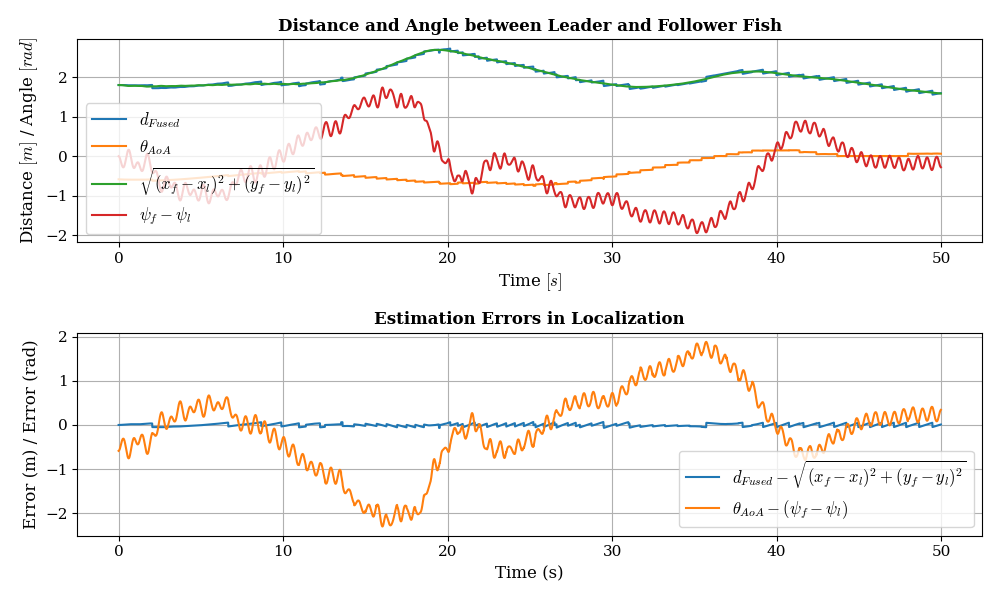
\includegraphics[width=0.5\textwidth]{fig/formation_errors.png}
    \caption{Distance between the leader and follower robotic fish and estimation errors during the formation control.}
    \label{fig:formation_errors}
\end{figure}

The upper subplot shows the distance $d_{\text{rss}}$ and the angle of approach $\theta_{\text{AoA}}$ estimated based on RSS alongside their ground-truth counterparts: the Euclidean distance $X_f - X_l$ and the heading difference $\psi_f - \psi_l$, respectively. 
The lower subplot presents the corresponding estimation errors:
\begin{eqnarray}
d_{error}&=&d_{\text{rss}} - \sqrt{(x_f - x_l)^2 + (y_f - y_l)^2}\\
\theta_{error}&=&\theta_{\text{AoA}} - (\psi_f - \psi_l).
\end{eqnarray}
The results demonstrate that the relative localization system maintains reasonably accurate estimates throughout the experiment. 
Although small fluctuations are present, particularly in angle estimates due to oscillatory tail motion, the system is able to track both relative position and orientation with acceptable error bounds.

\section{Conclusions and Future Work}
This paper presents a relative localization technique based on received signal strength (RSS) measurements from 433 MHz RF transceivers with multiple antennas. The RSS data are fused with inertial measurements from an onboard IMU using an Extended Kalman Filter (EKF) for state estimation. A proof-of-concept demonstration is carried out in a water tank using a leader-follower robotic fish scenario in a realistic simulation environment. A detailed analysis of the results is presented that highlights the effectiveness of the proposed method.
The proposed technique enables estimation of the relative position and orientation between agents with acceptable accuracy, making it well-suited for underwater swarm robotics applications such as environmental monitoring, search and rescue, and underwater mapping. Moreover, the approach is generalizable and can be extended to other swarm robotics domains, including aerial and terrestrial systems.
Future work may include the integration of additional sensing modalities, such as a magnetic compass or magnetometer, to improve the accuracy of yaw ($\psi$) estimation. This would enhance the robustness of the localization system, particularly in environments where inertial drift is significant.

 \begin{ack}
    % \textcolor{red}{Place acknowledgments here.}
    %\section*{Acknowledgments}
Study concept, oversight, and funding were provided by the U.S. Department of the Interior, Bureau of Safety and Environmental Enforcement (BSEE), Office of Offshore Regulatory Program Branch, Sterling, VA under Contract Number 140E0123C0007. The content, statements, findings, opinions, conclusions, and recommendations are those of the author(s) and do not necessarily reflect the views of the Bureau of Safety and Environmental Enforcement.
\end{ack}

\bibliography{ifacconf}           
\end{document}
